\beginsong{'k Heb mijn wagen volgeladen}
\beginverse*
'k Heb mijn wagen volgeladen,
Vol met oude wijven;
Toen ze op de marrekt kwamen,
Begonnen zij te kijven
Nu neem ik van mijn levensdagen
Geen oude wijven meer op mijn wagen!
Hop, paardje hop!
\endverse
\beginverse*
'k Heb mijn wagen volgeladen,
Vol met oude mannen
Toen zij op de marrekt kwamen,
Gingen ze samenspannen.
Nu neem ik van mijn levensdagen
Geen oude mannen meer op mijn wagen!
Hop, paardje hop!
\endverse
\beginverse*
'k Heb mijn wagen volgeladen,
Vol met jonge meisjes
Toen zij op de marrekt kwamen,
Zongen zij als sijsjes
Nu neem ik van mijn levensdagen
Steeds jonge meisjes op mijn wagen!
Hop, paardje hop!
\endverse
\endsong
\begin{intersong}
    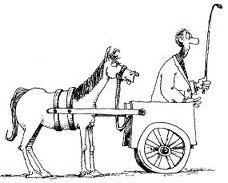
\includegraphics[width=0.4\textwidth]{img1}
\end{intersong}